% generation d'un .a que tu peux utiliser en ajoutant USE_STATIC_LIB=1 dans ton Makefile
% ajouter LDFLAGS+=-liio dans Makefile cree par module_generator

% device_reboot sf
% dfu-util -a firmware.dfu -D pluto.dfu

% dans le .dts : on remplace target = <&fpga_full>; par target = <&fpga_axi>; et on commente le nom du bitstream

\documentclass{article}
\usepackage{makeidx,anysize,mflogo,xspace,float,epsfig,url}
\usepackage{amsmath,amsfonts,amssymb,a4wide} 
\usepackage[utf8]{inputenc}
%\usepackage[francais]{babel}
%\usepackage[french]{babel}
\urlstyle{sf}
%\usepackage{subcaption}
\usepackage{hyperref}
\usepackage{graphicx}
\usepackage{graphics}
\usepackage{float}
\usepackage{caption}
\usepackage{colordvi} %??
\usepackage{listings} 
\usepackage{subfigure}
\usepackage{subfloat}
\usepackage{xcolor}
\graphicspath{{./figures/}}
%\usepackage[labelsep=quad,indention=10pt]{subfig}
\definecolor{grey}{rgb}{0.95,0.95,0.95} % on définit la couleur grise
	% (c'est un gris très clair)
	\definecolor{red}{rgb}{1.0,0.0,0.0} 
	\definecolor{green}{rgb}{0.0,1.0,0.0}
	\definecolor{blue}{rgb}{0.0,0.0,1.0}
	\lstloadlanguages{bash,Java,C,C++,csh,make,sh}%%[Visual]Basic,xml}
	\lstset{frame=none,basicstyle=\footnotesize,breaklines,tabsize=2,captionpos=b,
		prebreak={\hbox{$\rightarrow$}},postbreak={\hbox{$\hookrightarrow$}},
		showstringspaces=false,backgroundcolor=\color{grey}\bfseries,
		keywordstyle=\color{blue},commentstyle=\color{green}\textit,
		stringstyle=\color{red}\ttfamily,abovecaptionskip=2pt,aboveskip=0pt,
		belowskip=0pt,belowcaptionskip=0pt,numbers=none,columns=fullflexible, backgroundcolor=\color{grey}}
%left,numberstyle=\footnotesize,
%		stepnumber=2,numbersep=1pt}

\begin{document}


\begin{center}
{\bf \Large Using ADALM-PLUTO with the OscImpDigital Ecosystem} \\ \ \\
P.-Y. Bourgeois, G. Goavec-Merou, J.-M Friedt \\ 
\href{mailto:pyb2@femto-st.fr}{\{pyb2,gwenhael.goavec,jmfriedt\}\_at\_femto-st.fr}\ \\ \today
\end{center}


This tutorial is intended to help you to handle the ADALM-PLUTO (PlutoSDR) board within the
OscImpDigital framework.
It is focused on

\begin{itemize}
	\item Providing general guidelines to set up the environment
	\item Performing a PlutoSDR's harware independant check (NCO$\to$RAM, check the data)
	\item Connecting the PlutoSDR data stream into the RAM and recovering the data
\end{itemize}

\begin{figure}[h!]
	\centering{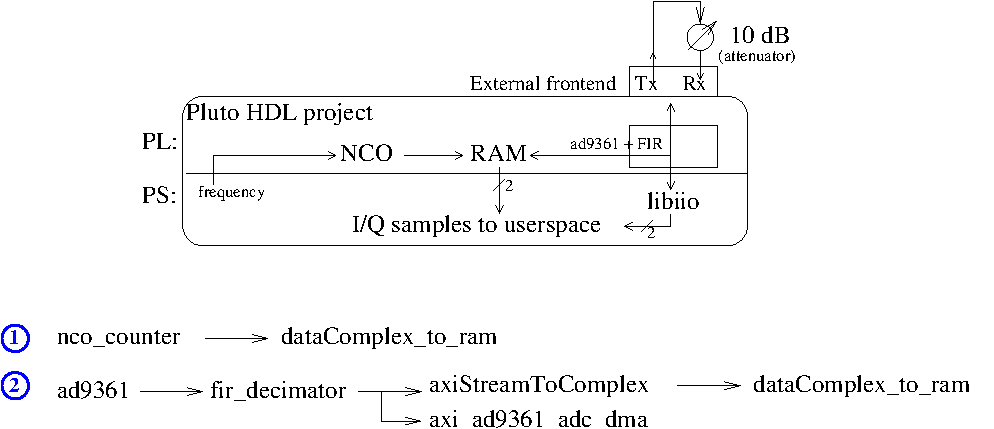
\includegraphics[width=\linewidth]{pluto-oscimpDigital-objective}
		\caption{Objectives of this tutorial and raw schematics of the
processing chains.}}
\end{figure}


%-----------------------------------
%\section*{Disclaimer}
%-----------------------------------
%Neither the author nor the developpers of the OscImpDigital repositories shall be
%responsible for misuse of the presented Software and Hardware.
%All the given codes and guidelines of this tutorial are provided ``as is''.

%-----------------------------------
\section{Objectives / Experimental set-up}
%-----------------------------------

Right out of the box, the ADALM-PLUTO board, when fired up, is able to be fully
configurable and flawlessly accessible thanks to the \emph{iio} contexts of {\bf{libiio}}.
Analog Devices Inc. (ADI) provides the library but also distributes the HDL code.
It becomes then interresting to test the compatibility of the original PlutoSDR HDL
project with the OscImpDigital ecosystem and benefit from extra features by pre-processing
the radiofrequency datastream on the high bandwith Programmable Logic (PL) FPGA of the
Zynq processor before transferring the lower bandwith dataset to the Processing System (PS).

For this tutorial, we want to recover I/Q samples of a 100~kHz beatnote. Achieving this
result is first assessed by fetching samples from the output of a 100~kHz NCO operating
independently of the AXI Stream provided by ADI. Having checked that the samples are
properly generated and recovered, we mix the output of the AXI Stream including the
I/Q coefficients from the AD9363 and check that the result is consistent. Thus:

\begin{itemize}
\item the first part aims at checking the correct bitstream synthesis of the project
provided by ADI using an additional NCO and RAM transfer from the OscImpDigital
ecosystem. In this setup (called sanity check), the NCO acts as a fake 100~kHz
beatnote generator, the added IPs having no relationship with the initial
firmware,
\item in the second part, we connect custom blocks to the AXI Stream from the
AD9363 and demonstrate how custom processing can be added to the original ADI processing chain.
\end{itemize}


In order to create a ``beatnote'', one can use the following setup:

%\begin{figure}[h!]
\begin{minipage}[c]{0.49\linewidth}
	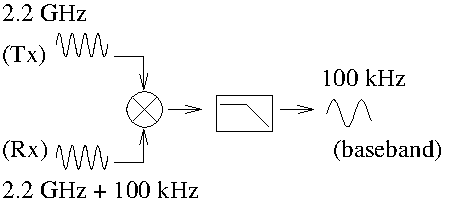
\includegraphics[width=\linewidth]{beatnote_pluto_scheme.pdf}
\end{minipage}\hfill
\begin{minipage}[c]{0.49\linewidth}
	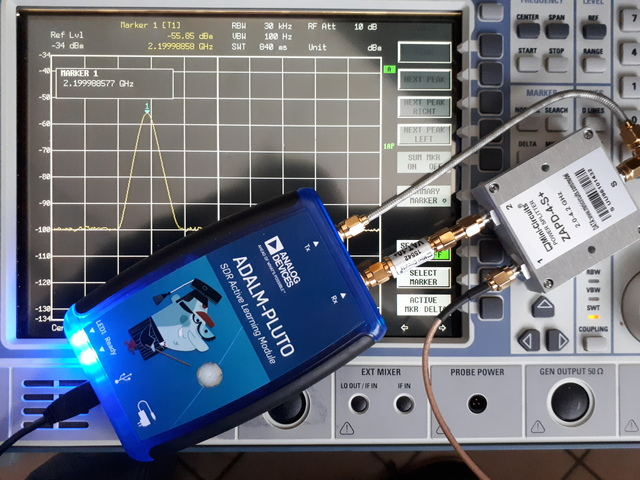
\includegraphics[width=\linewidth]{20190213_105039_640.jpg}
\end{minipage}
\vspace{0.1cm}
%\end{figure}

The {\bf Tx} port of the PlutoSDR board is set to transmit at 2.2~GHz. When connecting
the PlutoSDR Sink (select an input level lower than 1 to avoid saturation and 
unwanted signal beyond the carrier), the Tx transmits the unmodulated carrier at 2.2~GHz 
(i.e. with no signal of interrest nor message). The receiver part is slightly detuned at 
$2.2$~GHz$+100$~kHz. After demodulation (RF-hardware) and decimating filter ({\tt fir\_decimator}
block within the PL-side of the FPGA), a remaining ``beatnote'' at $f_b=100$~kHz occurs.
Once we know in advance the frequency of this beatnote, when the sampling rate
is set up at $fs=2$~MHz (as defined in the application to be discussed in section \ref{fs}
), we also know that a window 
of $N=2048$ samples will present $N\times fb/fs\simeq 102$~periods of the beatnote.
This ``beatnote'' trick is routinely used when developping
RF applications, to check that collected data are sound.

On the photography, a splitter has been added (before the 10~dB attenuator) to also send the 
{\bf Tx} port output to a spectrum analyzer which allows to check if the right carrier frequency 
has been set up through {\it iio}. 
% comprends pas le sens ci-dessous, comme on ne voit pas l'echelle de la courbe l'ecart entre
% TX LO et RX LO n'est pas visible ... ne me semble pas utile
%Obviously the peak measure does not show a $\sim$round 2.20 GHz
%frequency because the pluto and the spectrum analyzer embed different clocking
%systems that are further not referenced to an atomic reference.

%-----------------------------------
\section{Setting up the environment}
%-----------------------------------

Up to date versions of the following repositories must be fetched:
	\begin{itemize}
		\item The BR2\_EXTERNAL framework for Analog Device's PlutoSDR Zynq \\ (\href{https://github.com/oscimp/PlutoSDR}{https://github.com/oscimp/PlutoSDR}) and compile the Buildroot environment following the instructions
provided in the github repository {\tt README.md} file,
		\item The HDL project from Analog Devices (see further below).
In order to build the HDL project for the ADALM-PLUTO board, only the {\bf{hdl}} repository
(\href{https://github.com/analogdevicesinc/hdl}{https://github.com/analogdevicesinc/hdl}) is needed.
% but it is recommended to checkout the conservative commit used in
% \href{https://github.com/analogdevicesinc/plutosdr-fw}{https://github.com/analogdevicesinc/plutosdr-fw}. 
% JMF : je vire car inutile (cf hash ci-dessous en cas de doute)
		\item OscImpDigital (\href{https://github.com/oscimp/oscimpDigital}{https://github.com/oscimp/oscimpDigital}). Remember to recursively clone the repository\\
{\tt git clone --recursive https://github.com/oscimp/oscimpDigital} \\
			and set the {\tt BOARD\_NAME} to {\tt plutosdr} in the {\tt settings.sh} script. 
Although the PlutoSDR is fitted with the same Zynq model than
the Redpitaya, this variable will allow us to execute commands such as generating the DFU image or flashing
the embedded board. Furthermore, we will have to inform where the ADI HDL repository is located by defining the
{\tt ADI\_HDL\_DIR} variable in addition to {\tt BR\_DIR} indicating where the BuildRoot repository is located.
	\end{itemize}

\smallskip
At the time of writing (\today), the following versions are functional:
	\begin{itemize}
		\item {\bf{adi\_hdl}} branch {\bf{hdl\_2018\_r2}} (401395cdd1980827fd1f7043ce1a10770f666c64)
		\item Vivado 2018.3
	\end{itemize}

%-----------------------------------
\section{Sanity check (NCO$\to$RAM$\to$UserSpace)}
%-----------------------------------
This tutorial allows us to use the OscimpDigital blocks with the embedded Zynq of
the PlutoSDR board. It is seen as a first demonstration of compatibility.

\subsection{Design}

To build the HDL project for the PlutoSDR board, {\tt source} the
{\tt settings64.sh} script of Vivado 2018.2, the OscImpDigital
{\tt settings.sh}. Go to the first tutorial directory located in\\
{\tt oscimpDigital/doc/tutorials/plutosdr/1-adalmPluto\_within\_OscimpDigital}
and from the {\tt project1/design} sub-directory of this tutorial, run {\tt make xpr}.

A successful build of the HDL project is returned by the console message:\\
\noindent {\tt
Building {\bf{pluto}} project
[[...]/project1/design/pluto\_vivado.log] ... {\bf{OK}}
}

Once the pluto HDL project is successfully generated,
%built GGM
open \emph{pluto.xpr} within Vivado ({\tt vivado pluto.xpr}). 

%Add 
Check if the \emph{oscimpDigital/fpga\_ip} repository is present in the list of
IP repository (Icon ``Settings'' $\to$ ``Project
Settings'' $\to$ ``IP'' $\to$ ``Repository'' $\to$).% + then Apply and close the window).

Open the block design, right-click, ``Add IP'', then add the \emph{dataComplex\_to\_ram} 
and \emph{nco\_counter}. Run the ``Connection Automation'': the NCO counter and dataComplex\_to\_ram
should connect to the AXI bus and have addresses assigned to their registers: dataComplex\_to\_ram
base address should be 0x43C1\_0000 and nco\_counter base address should be 0x43C0\_0000. 
Refer to {\tt Address Editor} to verify, and if adresses mismatch, keep them in mind as you
will need it for the Device Tree overlay.

The next step is to configure the added IPs: %as shown in Fig. \ref{configs}, 
we set (double click on each block icon)
\begin{itemize}
\item the NCO block {\tt Data Size} to 16~bits, {\tt Counter Size} to 28~bits, and {\tt LUT
Size} to 10~bit,
\item the Data Complex to RAM block with {\tt Data Size} to 16~bits, {\tt Number of Inputs}
to 1, and {\tt Number of Samples} to 1024. % JMF/GGM : j'ai 1024 et non 2048 echantillons/voie
\end{itemize}

%\begin{figure}[h!]
%\begin{minipage}[c]{0.49\linewidth}
%	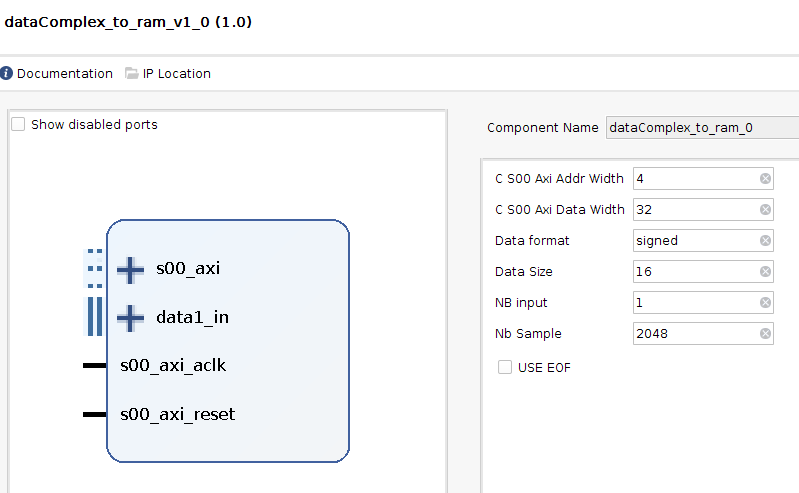
\includegraphics[width=\linewidth]{2019-02-12-165739_799x493_scrot.png}
%\end{minipage}\hfill
%\begin{minipage}[c]{0.49\linewidth}
%	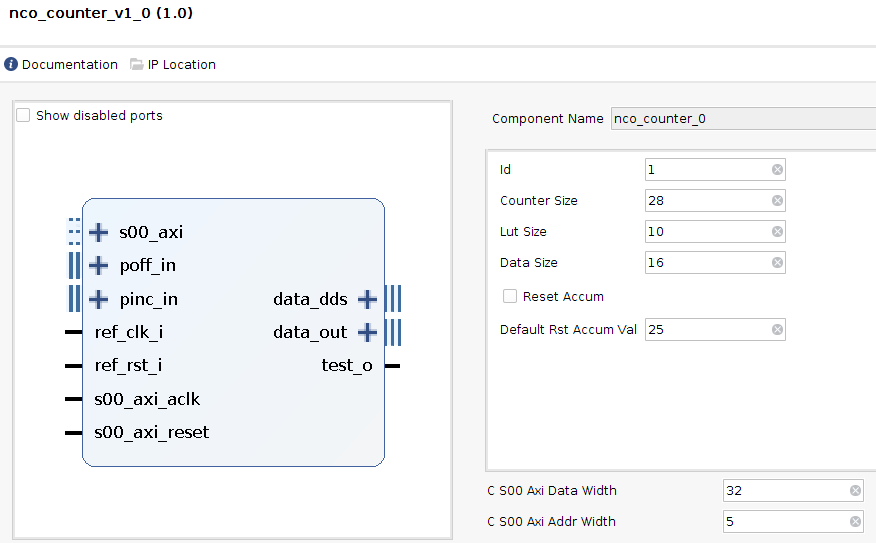
\includegraphics[width=\linewidth]{2019-02-12-170033_876x543_scrot.png}
%\end{minipage}
%\label{configs}
%\end{figure}

Additional connections (Fig. \ref{con}) for control signals:

\begin{itemize}
\item NCO
	\begin{itemize}
	\item {\tt ref\_rst\_i} $\to$ {\tt s00\_axi\_reset} on the same block
	\item {\tt ref\_clk\_i} $\to$ {\tt s00\_axi\_aclk} which refers to the PS7's
FCLK\_CLK0 at 100~MHz. We might as well clock and reset all blocks on the AD936x
signals (AD936x clock frequency depends on sampling frequency configured through
IIO API or GNURadio flowgraph).
	\end{itemize}
\item NCO $\to$ RAM
        \begin{itemize}
	\item {\tt sine\_out} $\to$ {\tt data1\_in} % JMF : changement de nom de la sortie
        \end{itemize}
\end{itemize}

\begin{figure}[h!tb]
%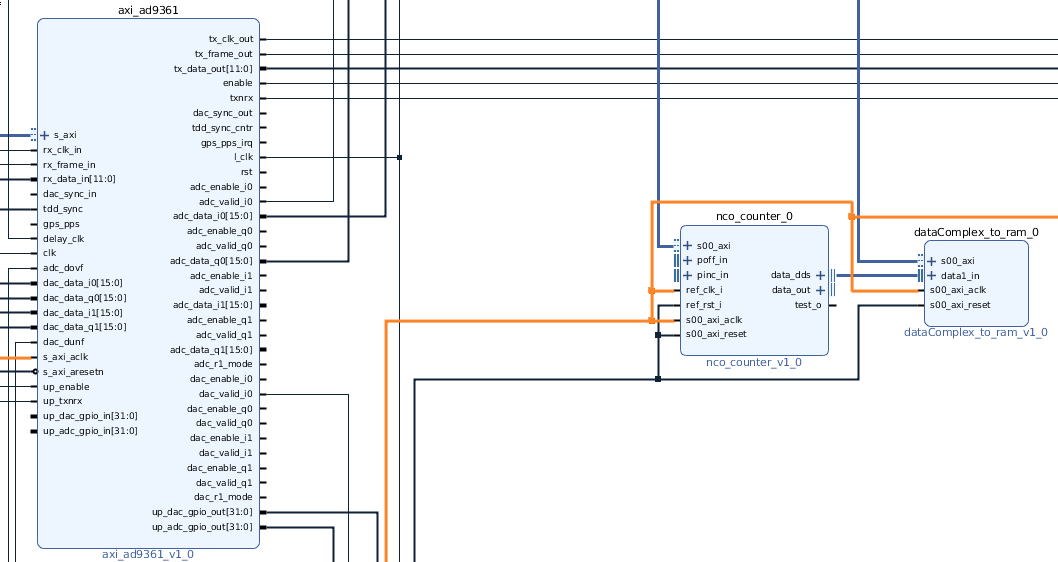
\includegraphics[width=.7\linewidth]{2019-03-07-091613_1058x562_scrot.png}%2019-02-12-171957_1072x583_scrot.png}
\begin{center}
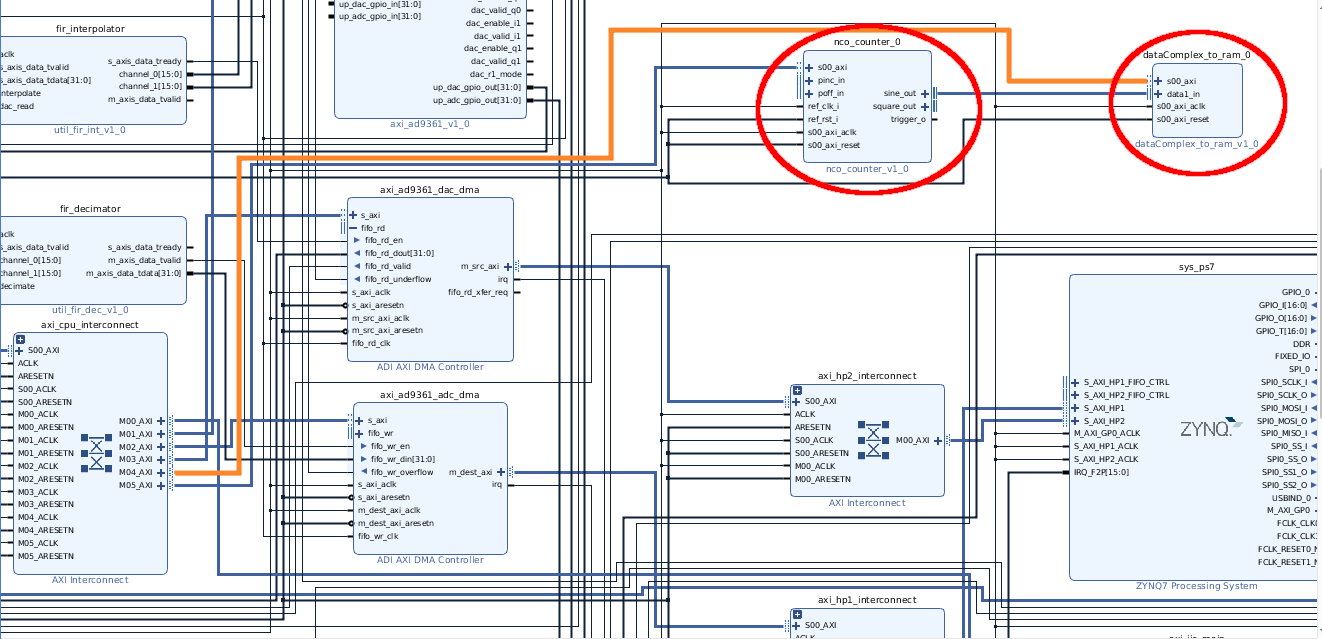
\includegraphics[width=\linewidth]{1.png}
\end{center}
\caption{Connection of the custom blocks to the PlutoSDR firmware.}
\label{con}
\end{figure}

At last, click on ``Generate Bitstream''.% and once the synthesis is done.%, place
%the {\tt /pathTo\_adi/hdl/projects/pluto/pluto.runs/impl\_1/system\_top.bit}
%into the \\{\tt /somewhere/PlutoSDR/board/pluto} BR2\_EXTERNAL directory.
%go back to terminal to use:
%\begin{lstlisting}
%make dfu_frm
%\end{lstlisting}
%to generate image/pluto.dfu and image/pluto.frm files.

Bistream generation is quite and lengthy task (depending on the host CPU). This time
is best spent compiling OscImpDigital libraries and drivers as well as creating
application for the PS as described in the next section.

%--------------------------------
\subsection{Preparing all OscimpDigital lib/driver/tools mandatories}
%--------------------------------

The NCO needs to be configured: rather than directly interacting with low level registers, the 
simpliest way is to benefit from the functions provided by the OscImpDigital library to do this task.

To build the library, go to {\tt \$OSCIMP\_DIGITAL\_LIB} and use the command:
\begin{lstlisting}
make
\end{lstlisting}
After that the current directory must contain two files: {\tt
liboscimp\_fpga.so} and {\tt liboscimp\_fpga\_static.a}: the latter can be linked with
an application by defining at {\tt USE\_STATIC\_LIB=1} option as will be discussed below.

Communications between PS userspace applications and IPs in the PL are achieved thanks
to Linux drivers. To build mandatory drivers go to {\tt \$OSCIMP\_DIGITAL\_DRIVER} and use
\begin{lstlisting}
make
\end{lstlisting}
as this command will iterate on all subdirectories and build each driver.

The last element to build is {\tt module\_generator}. This tool will be used to
build a skeleton for applications based on an XML description (see bellow).
Go to {\tt \$OSCIMP\_DIGITAL\_APP/tools/module\_generator} and again use
\begin{lstlisting}
make
\end{lstlisting}

%%GGM: a revoir 
%The library {\bf{liboscimp\_fpga}} should be compiled for your environment. We have selected
%to statically link the library to the application to avoid
%%GGM
%the need to reinstall library after each reboot:
%%confusion with multiple library
%%versions:
%% GGM: utile ?
%when compiling the userspace application using the {\tt Makefile} provided by
%{\tt module\_generator} (see below) by adding {\tt USE\_STATIC\_LIB=1} after the
%{\tt BASE\_NAME}
%
%Also both drivers for the NCO ({\tt nco\_counter\_core.ko}) and RAM ({\tt
%data\_to\_ram\_core.ko}) should be compiled. 

%--------------------------------
\subsection{Userspace application}
%--------------------------------

{\tt module\_generator}
(\url{https://github.com/oscimp/app/tree/master/tools/module_generator}) is used
to generates a skeleton for the application:
\begin{itemize}
\item {\tt Makefile} to cross-compile and install application and devicetree overlay;
\item devicetree source {\tt dts} file to inform the linux kernel about drivers to load and base memory
area to communicate with IP in PL;
\item script to prepare everything (load drivers and devicetree) before using
the binary application.
\end{itemize}

This tool uses a XML file which describes the list of IPs and its base address.
This file may contain options (if the OscImpDigital library is statically or
dynamically linked
or not used, if the application must be linked with others libraries, ...).

%The linux-side of the Pluto board uses the Device Tree overlays mechanism to
%affect the kernel side tree which allows for PL configuration dynamically.
%
%All we have to do is to indicate the presence of the NCO and RAM into the Device
%Tree structure. 
%A dirty but efficient way to do this is to edit the {\bf{zynq-pluto-sdr.dtsi}}
%that stands in \emph{/pathTo/buildroot-2018.11.1/output/build/linux-something/arch/arm/boot/dts/}
%
%%../../zynq-pluto-sdr.dtsi -> buildroot-2018.11.1/output/build/linux-c2041af164e263d852897cf90edb5cca9f677579/arch/arm/boot/dts/zynq-pluto-sdr.dtsi
%
%
%and eventually change the addresses accordingly:
%\begin{verbatim}
%
%/ {
%        fpga_axi: fpga-axi@0 {
%                compatible = "simple-bus";
%                #address-cells = <0x1>;
%                #size-cells = <0x1>;
%                ranges;
%
%                axi_i2c0: i2c@41600000 {
%
%...
%...
%
%                data2ram: data2ram@43c00000{
%                        compatible = "ggm,dataToRam";
%                        reg = <0x43c00000 0xffff>;
%                };
%
%                nco00: nco00@43c10000{
%                        compatible = "ggm,nco_counter";
%                        reg = <0x43c10000 0xffff>;
%                };
%
%        };
%};
%
%&spi0 {
%        status = "okay";
%...
%...
%\end{verbatim}

The configuration file ({\tt project1/module\_generator.xml}) for this first
application looks like
{
\begin{verbatim}
<?xml version="1.0" encoding="utf-8"?>
<project name="project1" version="1.0">
  <options>
    <option target="makefile" name="USE_STATIC_LIB">1</option>
    <option target="makefile" name="LDFLAGS">-liio</option>
  </options>
  <ips>
    <ip name="dataComplex_to_ram" >
      <instance name="data00" id="0" base_addr="0x43c10000" addr_size="0xffff" />
    </ip>
    <ip name="nco_counter" >
      <instance name="nco00" id="0" base_addr="0x43c00000" addr_size="0xffff" />
    </ip>
  </ips>
</project>
\end{verbatim}
%\begin{verbatim}
%<?xml version="1.0" encoding="utf-8"?>
%<drivers name="PlutoSDR_custom" version="1.0">
%  <driver name ="data_to_ram" >
%    <board_driver name="data00" id = "0" base_addr="0x43c10000" addr_size="0xffff" />
%  </driver>
%  <driver name ="nco_counter" >
%     <board_driver name="nco00" id = "0" base_addr="0x43c00000" addr_size="0xffff" />
%  </driver>
%</drivers>
%\end{verbatim}
}
where {\tt data00} and {\tt nco00} are the {\tt /dev} entries and the base addresses
should match those provided by Vivado.
The {\tt USE\_STATIC\_LIB} option is used to add a constant in the
{\tt Makefile} to specify that the static library should be linked with the
application and LDFLAGS
specify a dynamic link to the libiio since we will use IIO API to configure RF
frontends (see bellow).

The command:\\
{\tt \$OSCIMP\_DIGITAL\_APP/tools/module\_generator/module\_generator
module\_generator.xml}\\
will create a new directory called {\tt app} and fill it with the
{\tt Makefile}, a script called {\tt project1\_us.sh} and the {\tt dts} file {\tt
project1.dts}.
%GGM: obsolete
%A few updates must be brought to the output
%of {\tt module\_generator} after running {\tt module\_generator -dts config.xml}
%\begin{itemize}
%\item in dans le {\tt .dts}: replace \verb~target = <&fpga_full>;~ with \verb~target = <&fpga_axi>;~ 
%and comment out the bitstream name
%\item in the {\tt Makefile}, add {\tt USE\_STATIC\_LIB=1} and {\tt LDFLAGS+=-liio} after the project
%name but prior to the {\tt Makefile.inc} inclusion
%\item in the shell script, comment the lines creating the firmware directory and attempting to copy
%the bitstream to this location.
%\end{itemize}

The final task is to write the application behaviour {\tt project1/app/main.c}

The application-side makes use of \emph{libiio} as well as \emph{liboscimp}. For
the former, one can find examples from M. Hennerich presentation at GNU Radio Conference 2018
\footnote{
\href{https://www.gnuradio.org/grcon/grcon18/presentations/plutosdr/}{www.gnuradio.org/grcon/grcon18/presentations/plutosdr/}}
or following guidelines written in the ADI wiki website
\footnote{
\href{https://wiki.analog.com/resources/tools-software/linux-drivers/iio-transceiver/ad9361}{wiki.analog.com/resources/tools-software/linux-drivers/iio-transceiver/ad9361}}
\footnote{
\href{https://wiki.analog.com/university/tools/pluto/controlling\_the\_transceiver\_and\_transferring\_data}{wiki.analog.com/university/tools/pluto/controlling\_the\_transceiver\_and\_transferring\_data}}
to tweek the configuration.

For this part, we have just changed Hennerich's snippet code to the desired
configuration of TX and RX carriers, sampling rate, while the processing part only
consists in writing the RAM buffer into a data file.

\label{fs}
\begin{lstlisting}[language=C, numbers=left]
[...]
#include <iio.h> /* IIO API */
#include <nco_conf.h> /* NCO function */

#define ELEMENT_SIZE 1024	// Nb Sample

#define CLK_FREQ 2000000
#define MOD_FREQ 100000
#define NCO_ACCUM_SIZE 28

int main()
{
	int16_t *rawData;
	int ramfd = 0, i;

	struct iio_device *dev, *phy;
	struct iio_context *ctx;
	struct iio_channel *rx0_i, *rx0_q;

	rawData = (int16_t *) malloc(2 * ELEMENT_SIZE * sizeof(int16_t));

	ctx = iio_create_local_context();

	dev = iio_context_find_device(ctx, "cf-ad9361-lpc");
	phy = iio_context_find_device(ctx, "ad9361-phy");

	iio_channel_attr_write_longlong(iio_device_find_channel(phy, "altvoltage1", true),
		"frequency", 2200000000);	/* TX LO frequency 2.4GHz */

	iio_channel_attr_write_longlong(iio_device_find_channel(phy, "altvoltage0", true),
		"frequency", 2200100000);	/* RX LO frequency 2.4GHz + 100 kHz */

	iio_channel_attr_write_longlong(iio_device_find_channel(phy, "voltage0", false),
		"sampling_frequency", CLK_FREQ);	/* RX baseband rate 2 MSPS */

	rx0_i = iio_device_find_channel(dev, "voltage0", 0);
	rx0_q = iio_device_find_channel(dev, "voltage1", 0);

	iio_channel_enable(rx0_i);
	iio_channel_enable(rx0_q);

	/* NCO configuration */
	nco_counter_send_conf("/dev/nco00", CLK_FREQ, MOD_FREQ,
			      NCO_ACCUM_SIZE, 0, 1, 1); // 0, 1, 1 => offset, PINC HW/SF, POFF HW/SF

	ramfd = open("/dev/data00", O_RDONLY);
	if (ramfd < 0) {
		perror("ram open error\n");
		return EXIT_FAILURE;
	}
	read(ramfd, rawData, 2 * ELEMENT_SIZE * sizeof(int16_t));
	FILE *fd = fopen("data.dat", "w");
	for (i = 0; i < 2 * ELEMENT_SIZE; i+=2)
		fprintf(fd, "%d %d\n", rawData[i], rawData[i+1]);
	fclose(fd);
	close(ramfd);
	iio_context_destroy(ctx);
	free(rawData);
	return EXIT_SUCCESS;
}
\end{lstlisting}

The most important lines for this first project where we only fetch the data
stream produce by the NCO are:
\begin{itemize}
\item lines 33-34: set the sample frequency (here 2~MS/s for consistency, although
sampling rates up to 64~MS/s can be achieved between the AD9363 and the Zynq). This frequency
corresponds to the {\tt l\_clk} output from {\tt axi\_ad9361} IP and is used by the
NCO though {\tt ref\_clk} input for clocking frequency.
\item lines 43-44: {\tt nco\_counter\_send\_conf} is the OscImpDigital library
function to configure the NCO IP. We found:
\begin{itemize}
\item a {\tt /dev/nco00} according to the
dev name provided in the XML file;
\item the same constant used to configure the sampling frequency and here specifying the
IP clocking frequency to compute phase increment work;
\item the output, requested, frequency corresponding to the beatnote between TX
LO frequency and RX LO frequency;
\item the phase accumulator size again used to compute the phase increment;
\item and, but out of the scope of this tutorial, a phase offset, and a mux
configuration to driver phase increment and offset from AXI or from NCO IP
inputs
\end{itemize}
\item finally lines 46-51: the {\tt /dev/data00} is opened and a simple read is
used to fetch samples from data stream. we read 16bits $\times 1024 \times 2$
(the $\times 2$ is due to the complex I/Q samples)
\end{itemize}

{\tt make} will produce both {\tt project1.dtbo} and {\tt project1\_us}.

%--------------------------------
\subsection{Update PlutoSDR firmware and install application}
%--------------------------------

Now we have a {\tt .bit} for the PL and application for the PS.

First a new firmware image must be produced containing the custom bitstream. In
the {\tt design} directory the command {\tt make dfu\_frm} will produce both {\tt .dfu}
and {\tt .frm} images.

Two firmware flashing strategies can be followed:
\begin{itemize}
\item using the {\tt .frm}, we copy the file to the PlutoSDR mass storage and reboot by:
	\begin{itemize}
	\item {\tt sudo mount /dev/sdx /mnt/sd} (see {\tt dmesg} for corresponding device)
	\item {\tt cp image/pluto.frm /mnt/sd}
	\item {\tt sudo eject /dev/sdx}
	\end{itemize}
	You should see the {\bf \textcolor{blue}{blue LED1}} flashing quickly: {\bf do not disconnect
	nor touch anything until the PlutoSDR has rebooted} or you may brick the board at
	this stage. 
\item using the {\tt .dfu:} use the command {\tt make flash\_dfu\_frm} to reboot the
board in dfu mode (password will be asked: analog) and to flash the {\tt pluto.dfu} image. This
option is prefered for large images which sometimes do not fit in the remaining mass storage space.

	When {\tt dfu-util} displays:
	\begin{verbatim}_firmware
Copying data from PC to DFU device
Download        [=========================] 100%     30669815 bytes
Download done.
state(7) = dfuMANIFEST, status(0) = No error condition is present
state(2) = dfuIDLE, status(0) = No error condition is present
Done!
	\end{verbatim}
	unplug and replug the PlutoSDR.
\end{itemize}

%The last step is then to rebuild the firmware ({\tt pluto.frm}) :
%
%\begin{itemize}
%	\item remember that we have copied the bitstream to the PlutoSDR
%directory in \\
%{\tt /somewhere/PlutoSDR/board/pluto}, hence providing buildroot with the appropriate
%bitstream named {\tt system\_top.bit}.
%	\item {\tt cd pathTo/buildroot-version/}
%	\item {\tt make}
%\end{itemize}
%
%\paragraph{NB:} For the moment, the repository PlutoSDR provides only support
%for rootfs and linux (the bootloader part still remains to be added). Hence, any
%change of the bistream requires to perform the steps presented here:
%
%\begin{itemize}
%	\item Fire up the PlutoSDR // wait for the mass-storage to be available (via
%{\tt dmseg -w} for example)
%	\item {\tt mount /dev/sdX1\footnote{X is the index of the pluto mass-storage, e.g.
%/dev/sde1} /mnt/somewhere/}
%	\item {\tt cp pathTo/buildroot-version/output/images/pluto.frm /mnt/somewhere/}
%	\item {\tt eject /dev/sdX1}  % JMF : moi j'ai toujours fait sdX : est-ce correct ?
%\end{itemize}


%Alternatively, the DFU image can be transfered to the PlutoSDR flash by rebooting,
%from the target GNU/Linux prompt, to DFU mode with
%{\footnotesize
%\begin{verbatim}
%device_reboot sf
%\end{verbatim}
%}
%and then running on the host personnal computer
%{\footnotesize
%\begin{verbatim}
%dfu-util -a firmware.dfu -D my_pluto_firmware.dfu
%\end{verbatim}
%}
%with {\tt my\_pluto\_firmware.dfu} matching the name of the image to be flashed. Again wait for
%the transfer to complete and the message stating that no error was detected to appear.
%
Now that the firmware including the updated bitstream has been flashed, the PlutoSDR is ready to be tested.

In the {\tt app} directory use:
\begin{lstlisting}
make install_ssh
\end{lstlisting}
Again, the PlutoSDR root password ({\tt analog}) is required.

To test the application:
\begin{lstlisting}
ssh root@192.168.2.1
\end{lstlisting}
and go to the directory in which the applications were stored, namely a sub-directory of {\tt /tmp}:
\begin{lstlisting}
cd /tmp/project1/bin/
\end{lstlisting}

%--------------------------------
\subsection{Testing the application}
%--------------------------------

%An example file is provided in the folder {\bf{get\_data/nco\_data2ram}}. Running this example
%requires loading the devicetree overlay and the kernel modules: all operations are taken care
%of by the bash script in the application directory. The {\tt dmesg} output should display
%something like

Before using the application, dtbo overides must be applied and drivers loaded:
this is done by executing {\tt ./project1\_us.sh}. The command {\tt dmesg} must
display something like:
{
\begin{verbatim}
[...]
data_to_ram_core: loading out-of-tree module taints kernel.                     
probing data00 with dts                                                         
name: data00 4 6                                                                
dataToRam 43c00000.data00: data00: Add the device to the kernel, connecting cde 
dataToRam 43c00000.data00: 6data00 loaded                                       
probing nco00                                                                   
name: nco00 4 5                                                                 
nco_counter 43c10000.nco00: nco00: Add the device to the kernel, connecting cde 
nco_counter 43c10000.nco00: 6nco00 loaded                                       
\end{verbatim}
}
with the first two lines exhibiting kernel messages resulting from the bitstream loading, then the
{\tt data\_to\_ram} driver and the {\tt nco} driver. The two {\tt /dev/nco00} and {\tt /dev/data00}
defined in the devicetree source should have been created.

Now launch {\tt ./project1\_us}: the {\tt /dev/data00} device is opened, the output
of the NCO fed to this block read from the PS, and stored in a file. Plotting the resulting
dataset yields charts similar to those shown in Fig. \ref{nco}.

% JMF : je ne comprends pas : l'exemple consiste a mesurer un NCO, et l`a je vois
%  des donnees bruit'ees. Ca ne colle pas avec mes mesures qui montrent un NCO "propre"
\begin{figure}[h!tb]
%\begin{minipage}[c]{0.49\linewidth}
%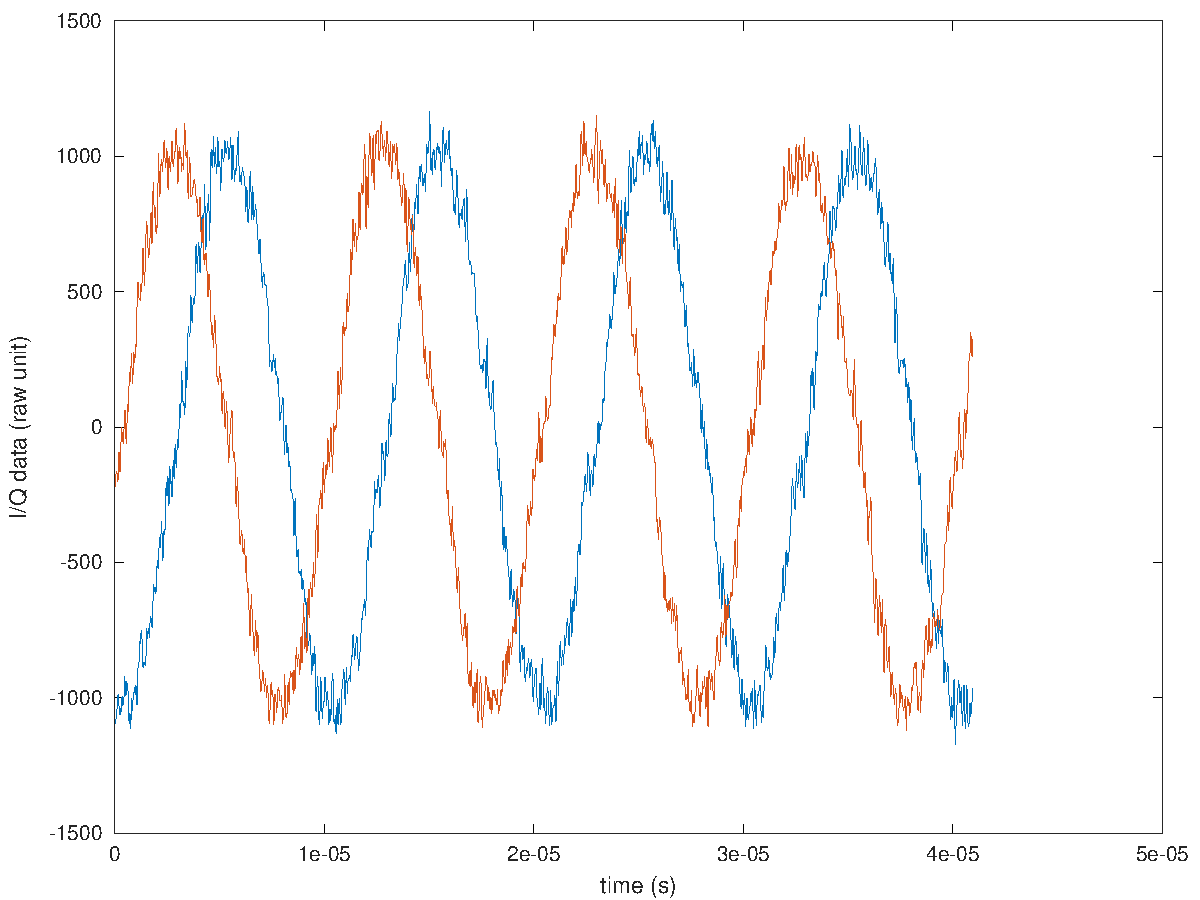
\includegraphics[width=\linewidth]{iio_iq_data.pdf}
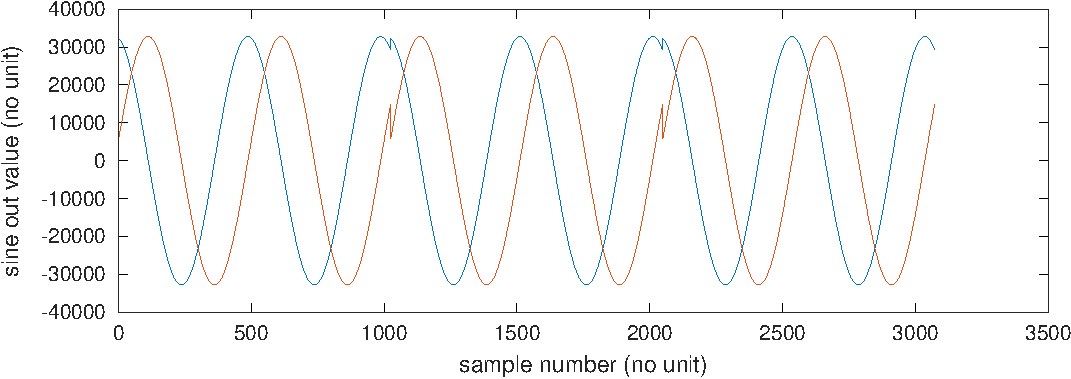
\includegraphics[width=\linewidth]{NCO.pdf}
%\end{minipage}\hfill
%\begin{minipage}[c]{0.49\linewidth}
%	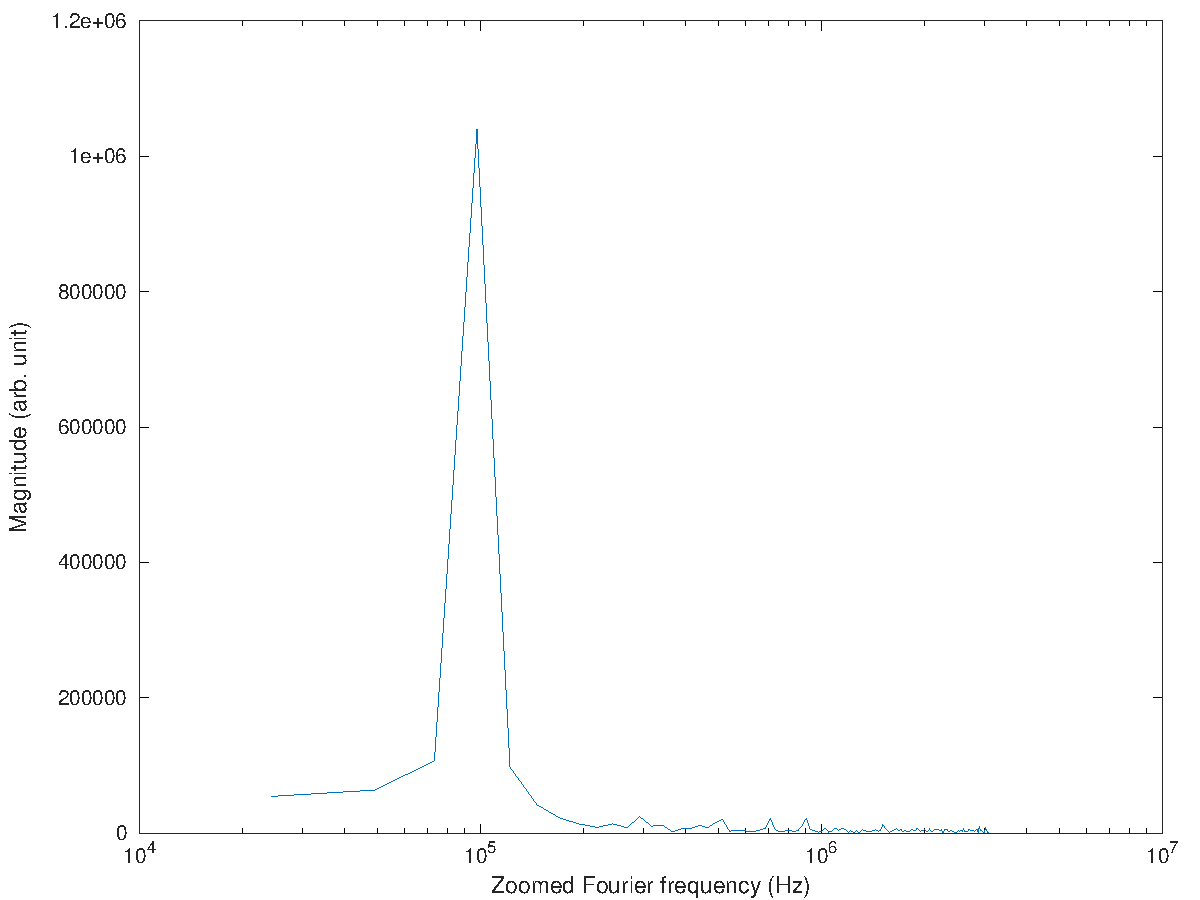
\includegraphics[width=\linewidth]{iio_fft_iq_data.pdf}
%\end{minipage}
\caption{Collected I/Q datasets. The 200~samples/period match the expected sampling
rate of 2~MS/s as a 100~kHz sine wave is generated by the NCO. Three successive (discontinuous)
datasets were collected.}% Right: Fourier transform.}
\label{nco}
\end{figure}

%-------------------------------------------------------
\section{PlutoSDR data stream $\to$ RAM $\to$ Userspace}
%-------------------------------------------------------
\subsection{Design update}
This second tutorial is a demonstration of the compatibility of the OscImpDigital
ecosystem with the use of the existing Pluto HDL.
Once complete, you should be able to plug any DSP task to the initial design and
perform extra processing chains (Figs. \ref{chain1} and \ref{chain2}).

\begin{figure}[h!tb]
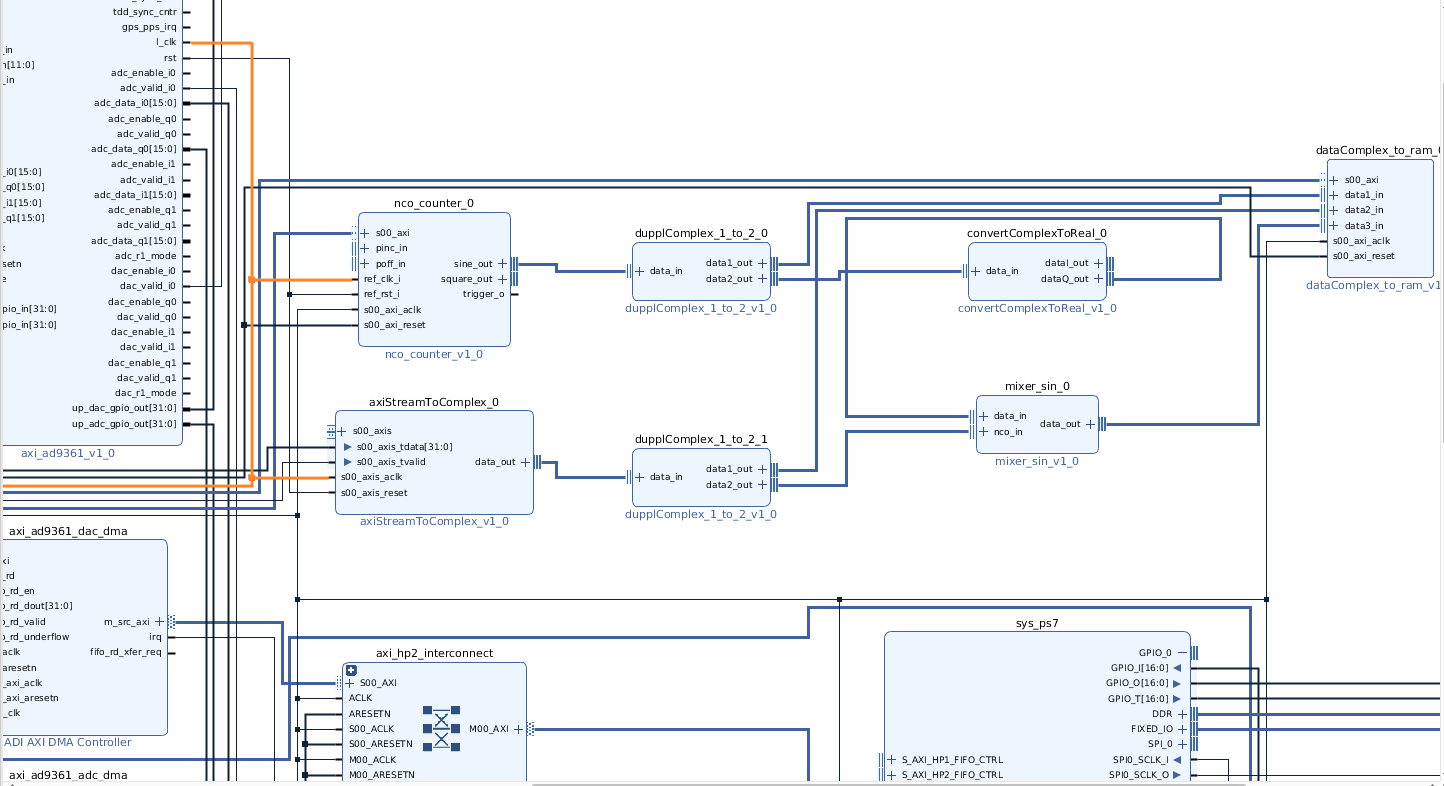
\includegraphics[width=\linewidth]{2.png}
\caption{Signal processing chain as defined in the Vivado 2018.3 graphical user
interface (added blocks are on the top right and include the nco\_counter, 
axiStreamToComplex, two duppComplex, convertComplextoReal, mixer\_sin and 
finally dataComplex\_to\_ram).}
\label{chain1}
\end{figure}

This project is an update of the previous one. Instead of only fetching data
stream generated by the NCO, we will use this data flow to frequency transpose the AD9361
data stream by mixing. A second update is to be done:
three datastreams lead to the DataToRAM block: the (complex) NCO output as addressed 
previously, the raw ADC (complex) data resulting from the I/Q demodulation within 
the AD9363 RF frontend, and the output of the mixer of the NCO with the ADC I/Q stream.

This time, since data from the AD9363 will be used in the flow chart, a consistent
clocking and signal reset distribution must be used:
\begin{itemize}
\item connect {\tt ref\_clk\_i} of the {\tt nco\_counter} to the {\tt axi\_ad9361} IP
{\tt l\_clk} (as is the {\tt s00\_axis\_aclk} of the {\tt axiStreamToComplex} block)
\item connect {\tt ref\_rst\_i} of the {\tt nco\_counter} to the {\tt axi\_ad9361} IP
{\tt rst} (as is the {\tt s00\_axis\_reset} of the {\tt axiStreamToComplex} block)
\item these clock and reset signals are then propagated to the other processing blocks through
their interfaces.
\end{itemize}

Failing to use these connections will result in timing errors including negative WNS and TNS
values related to the fact that the mixer is fed data from two different clock domains -- 100~MHz
for the AXI bus and 50~MHz for the AD9361.

We must add these IPs:
\begin{itemize}
\item {\em axiStreamToComplex}: since ADI IP uses AXI Stream interfaces and OscImpDigital custom real
	or complex interfaces, this IP must be used to convert interfaces.
	According to the RF frontend bus size, this block must be configured with
	{\tt Data Size = 16};
\item $2 \times$ {\em dupplComplex\_1\_to\_2}: when connection between two IPs is done
	using interfaces (instead of manually connecting wire/bus contained in an
	interface) a relation 1 to many is forbidden. The dupplXX IP acts as a splitter
	to copy inputs to both ouput ports. These two IPs must configured with
	{\tt Data Size = 16};
\item {\em mixerComplex\_sin}: this IP is used to apply a complex multiplication
	between the two input port data flow. This IP must be configured with {\tt
	Data Size = 16} according to the RF frondend size, and {\tt Nco Size = 16}
	according to the NCO configuration. 
\end{itemize}

Now it is time to connect blocks, but before that the connection between
{\tt NCO} and {\tt dataComplex\_to\_ram} set previously must be suppressed and the {\tt
dataComplex\_to\_ram} configuration must be modified to change {\tt NB input} to
3.

For connecting:
\begin{itemize}
\item {\tt fir\_decimator} $\to$ {\tt axiStreamToComplex}: click on {\tt '+'} before
{\tt axiStreamToComplex} {\tt s00\_axis} interface to expose all signals included in
this interface. Connect:
	\begin{itemize}
	\item {\tt fir\_decimator} {\tt m\_axis\_data\_tdata} $\to$ {\tt
	axiStreamToComplex} {\tt s00\_axis\_tdata};
	\item {\tt fir\_decimator} {\tt m\_axis\_data\_tvalid} $\to$ {\tt
	axiStreamToComplex} {\tt s00\_axis\_tvalid}
	\end{itemize}
\item {\tt axiStreamToComplex} $\to$ {\tt dupplComplex\_XX\_0}: connect {\tt
axiStreamToComplex} {\tt data\_out} $\to$ {\tt dupplComplex\_XX\_0} {\tt
data\_in};
\item {\tt nco\_counter} $\to$ {\tt dupplComplex\_XX\_1}: connect {\tt
nco\_counter} {\tt sine\_out} $\to$ {\tt dupplComplex\_XX\_1} {\tt
data\_in};
\item {\tt dupplComplex\_XX\_0} $\to$ {\tt mixerComplex}: connect
{\tt dupplComplex\_XX\_0} {\tt data1\_out} $\to$ {\tt mixerComplex} {\tt
data\_in};
\item {\tt dupplComplex\_XX\_1} $\to$ {\tt mixerComplex}: connect
{\tt dupplComplex\_XX\_1} {\tt data1\_out} $\to$ {\tt mixerComplex} {\tt
nco\_in};
\item {\tt dupplComplex\_XX\_0} $\to$ {\tt dataComplex\_to\_ram}: connect
{\tt dupplComplex\_XX\_0} {\tt data2\_out} $\to$ {\tt dataComplex\_to\_ram} {\tt
data1\_in};
\item {\tt dupplComplex\_XX\_1} $\to$ {\tt dataComplex\_to\_ram}: connect
{\tt dupplComplex\_XX\_1} {\tt data2\_out} $\to$ {\tt dataComplex\_to\_ram} {\tt
data2\_in};
\item {\tt mixerComplex\_sin} $\to$ {\tt dataComplex\_to\_ram}: connect
{\tt mixerComplex\_sin} {\tt data\_out} $\to$ {\tt dataComplex\_to\_ram} {\tt
data3\_in};
\end{itemize}

Additional connections for clock and reset signals:
\begin{itemize}
\item {\tt axiStreamToComplex} {\tt s00\_axis\_aclk} $\to$ {\tt axi\_ad9361}
{\tt l\_clk};
\item {\tt axiStreamToComplex} {\tt s00\_axis\_reset} $\to$ {\tt axi\_ad9361}
{\tt rst};
\end{itemize}

\begin{figure}[h!tb]
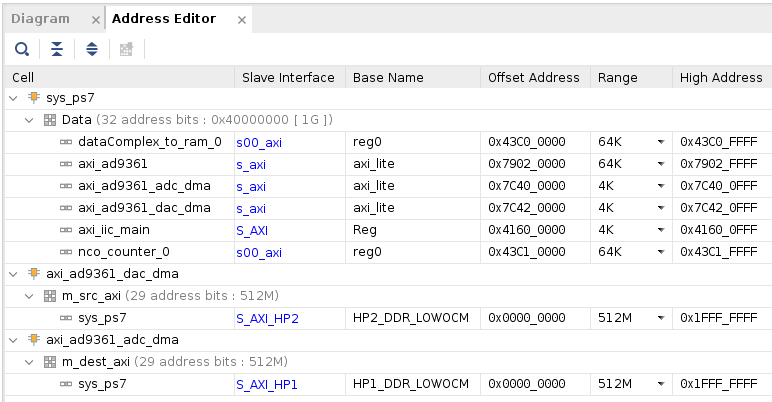
\includegraphics[width=\linewidth]{address.png}
\caption{Address map generated by Vivado: the devicetree source file must match
this configuration for the Linux drivers to reach registers at the right addresses.}
\label{chain2}
\end{figure}

Once these modifications are done, click on {\tt Generate bitstream} and switch to
application update while {\em Vivado} is working.

%Since the ADI ADC is fed to a FIR decimator with no interface on the AXI Stream bus,
%a direct connection to the axiStreamToComplex block is possible. Since the complex
%valued output exhibits an interface, the resulting stream must be dupplicated 
%(dupplCompl) when multiple processing -- here communication and mixing -- are to be
%performed on the complex valued datastreams.

\subsection{Application update}

Compared to the design, updates to apply to the PS part is small:
\begin{itemize}
\item since we want to feedback TX RF signal to the RX RF input, we will use
GNU Radio on the host computer to handle TX stream and to configure the {\em
AD936x} so we must remove all lines related to the RF frontend configuration
though IIO in the C source code.
\item using USB communication is a bottleneck, which is the reason why since the
beginning of this tutorial we have selected a sampling frequency if 2~MS/s. This
setting must be applied to the GNU Radio flowchart {\tt samp\_rate}. Check that this value
is selected as NCO clock frequency ({\tt \#define CLK\_FREQ});
\item in the previous project, {\tt dataComplex\_to\_ram} stored and transmitted 1
channel, 1024 $\times$ 16~bit complex integers. In this design update we have 3 input
channels. All references to buffer sizes must be updated accordingly.
\end{itemize}

\subsection{Testing}

Flashing firmware and application install to the PlutoSDR are exactly the same as
previously, so please refer to this section.

The resulting datasets are plotted on Fig. \ref{openclosed}, left with the
PlutoSDR disconnected from its input (noise measurement on the ADC) and right with
the RF output connected to the input through a 10~dB attenuator.

\begin{figure}[h!tb]
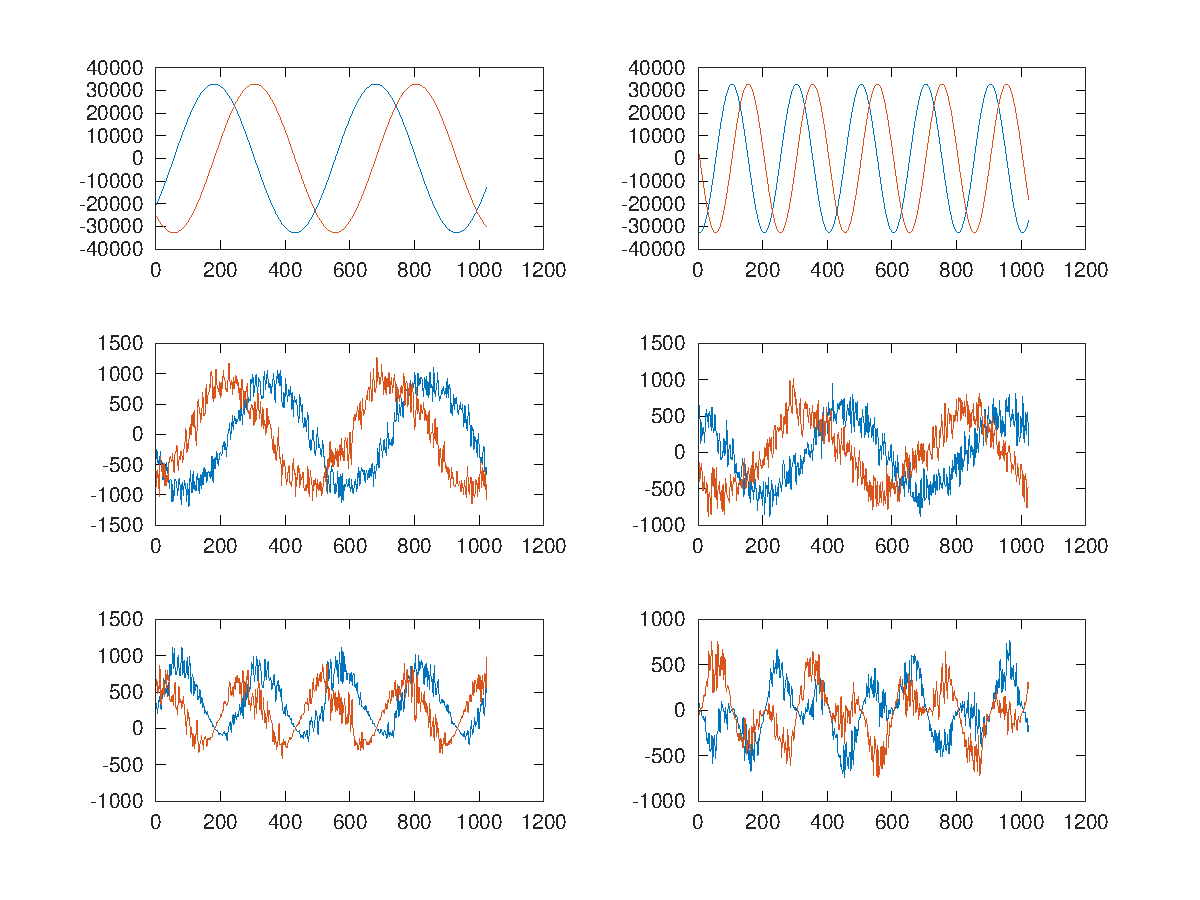
\includegraphics[width=\linewidth]{100kHz_250kHz}
\caption{Measurements results with a 100~kHz local oscillator (left) and with (right) a
250~kHz local oscillator, while in both cases the output is offset by 100~kHz from the
input. Top to bottom: NCO, measured I/Q streams, and mixer output.}
\label{openclosed}
\end{figure}

The original PlutoSDR used with GNU Radio remains functional despite the updated bitstream.
The same result than the one demonstrated from the OscimpDigital framework but running on the
host computer is shown in Fig. \ref{gnuradio}.

\begin{figure}[h!tb]
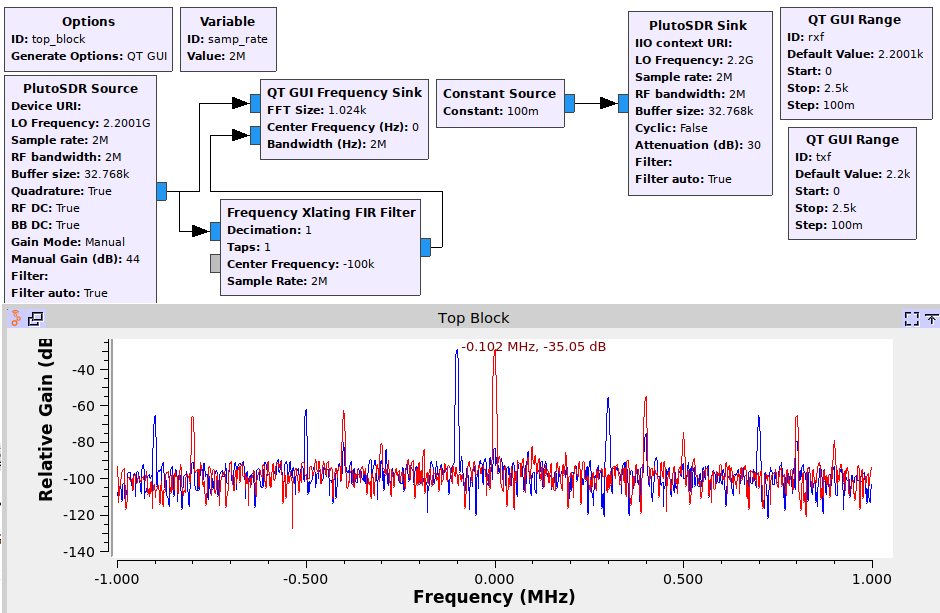
\includegraphics[width=\linewidth]{gnuradio.png}
\caption{GNU Radio flowchart accessing the PlutoSDR as source and sink with the updated
bitstream configuring the PL.}
\label{gnuradio}
\end{figure}

\section{TCL update of the original ADI PL configuration}

Rather than bothering with the graphical user interface, adding new functionalitites
brought by the OscimpDigital framework to the original ADI PL configuration file is most
efficiently achieved by updating the TCL script.

A default design for PlutoSDR, with OscimpDigital support, is available in the
tutorial subdirectory
{\tt project2/design} or alternatively in
{\tt \$OSCIMP\_DIGITAL\_APP/plutosdr/plutosdr\_template}.

%The TCL script provided by ADI is located at {\tt /somewhere/hdl/projects/pluto/system\_bd.tcl} and
%must updated with the following:
The TCL script must be updated with the additional blocks:

%\begin{itemize}
%\item at the beginning of the file, insert the location of the OscimpDigital IP repository with
%{\footnotesize
%\begin{verbatim}
%variable fpga_ip    $::env(OSCIMP_DIGITAL_IP)
%set_property  ip_repo_paths [list ${fpga_ip} ${lib_dirs}] [current_project]
%update_ip_catalog
%\end{verbatim}
%}
%\item append the design with the additional blocks:
{
\begin{verbatim}
# axiStreamToComplex
ad_ip_instance axiStreamToComplex axis2Complex
ad_ip_parameter axis2Complex CONFIG.DATA_SIZE 16

ad_connect axi_ad9361/rst axis2Complex/s00_axis_reset
ad_connect axi_ad9361/l_clk axis2Complex/s00_axis_aclk

ad_connect fir_decimator/m_axis_data_tdata axis2Complex/s00_axis_tdata
ad_connect fir_decimator/m_axis_data_tvalid axis2Complex/s00_axis_tvalid

#nco
ad_ip_instance nco_counter nco
ad_ip_parameter nco CONFIG.DATA_SIZE 16
ad_ip_parameter nco CONFIG.COUNTER_SIZE 28
ad_ip_parameter nco CONFIG.LUT_SIZE 10

ad_connect axi_ad9361/rst nco/ref_rst_i
ad_connect axi_ad9361/l_clk nco/ref_clk_i

ad_connect sys_rstgen/peripheral_reset nco/s00_axi_reset
ad_cpu_interconnect 0x43C00000 nco

# duppl raw data -> mixer and dataComplex_to_ram
ad_ip_instance dupplComplex_1_to_2 duppl_0
ad_ip_parameter duppl_0 CONFIG.DATA_SIZE 16

ad_connect axis2Complex/data_out duppl_0/data_in

# duppl NCO -> mixer and dataComplex_to_ram
ad_ip_instance dupplComplex_1_to_2 duppl_1
ad_ip_parameter duppl_1 CONFIG.DATA_SIZE 16

ad_connect nco/sine_out duppl_1/data_in

# mixer
ad_ip_instance mixerComplex_sin mixer
ad_ip_parameter mixer CONFIG.NCO_SIZE 16
ad_ip_parameter mixer CONFIG.DATA_SIZE 16

ad_connect duppl_0/data1_out mixer/data_in
ad_connect duppl_1/data1_out mixer/nco_in

#dataComplex
ad_ip_instance dataComplex_to_ram data_to_ram
ad_ip_parameter data_to_ram CONFIG.NB_INPUT 3
ad_ip_parameter data_to_ram CONFIG.DATA_SIZE 16
ad_ip_parameter data_to_ram CONFIG.NB_SAMPLE 1024

ad_connect duppl_0/data2_out data_to_ram/data1_in
ad_connect duppl_1/data2_out data_to_ram/data2_in
ad_connect mixer/data_out data_to_ram/data3_in

ad_connect sys_rstgen/peripheral_reset data_to_ram/s00_axi_reset
ad_cpu_interconnect 0x43C10000 data_to_ram

\end{verbatim}
}

TCL functions starting with {\em ad\_} are from ADI's {\tt hdl} repository:
\begin{itemize}
\item {\tt ad\_ip\_instance} is used to add an instance of an IP. The first
parameter is the name of the IP (not the {\em VLNV} ({\em Vendor Library Name
Version}) and the second is the instance name;
\item {\tt ad\_ip\_parameter} configures, for one instance whose name is given
as first argument, one parameter (second argument) with name
{\em CONFIG.XXX} with the value passed as third argument;
\item {\tt ad\_connect} to connect signals/interfaces between IPs with format
{\em instance\_name/interface\_name};
\item {\tt ad\_cpu\_interconnect} to connect the {\tt AXI Lite} interface for an
instance (second argument) to the Zynq PS, with base address provided as first
parameter.
\end{itemize}

Note: ADI {\tt ad\_cpu\_interconnect} automatically connects AXI clock and AXI
reset to the CPU, if this was not done previously. However, this function always
considers reset as active low. When the reset signal
is active high, as for most of OscImpDigital IPs, this signal must be {\bf explictly
connected} before using this function.

The most difficult aspect with this approach is to know interface names and
parameters: see {\tt \$OSCIMP\_DIGITAL\_IP/README.md} for a detailed description of each IP.
%\item update the {\tt Makefile} by removing
%{\footnotesize
%\begin{verbatim}
%M_DEPS += ../../library/xilinx/common/ad_iobuf.v
%M_DEPS += ../../library/axi_ad9361/axi_ad9361_delay.tcl
%\end{verbatim}
%}
%and replacing with
%{\footnotesize
%\begin{verbatim}
%M_DEPS += $(ADI_HDL_DIR)/library/xilinx/common/ad_iobuf.v
%M_DEPS += $(ADI_HDL_DIR)/library/axi_ad9361/axi_ad9361_delay.tcl
%\end{verbatim}
%}
%with {\tt ADI\_HDL\_DIR} set to the {\tt /somewhere/hdl/} location,
%\item 
%in the {\tt Makefile}, remove
%{\footnotesize
%\begin{verbatim}
%include ../scripts/project-xilinx.mk
%\end{verbatim}
%}
%and replace with
%{\footnotesize
%\begin{verbatim}
%include $(ADI_HDL_DIR)/projects/scripts/project-xilinx.mk
%\end{verbatim}
%}
%\item in the {\tt system\_project.tcl}, replace
%{\footnotesize
%\begin{verbatim}
%source ../scripts/adi_env.tcl
%\end{verbatim}
%}
%with
%{\footnotesize
%\begin{verbatim}
%variable adi_hdl_dir $::env(ADI_HDL_DIR)
%source $adi_hdl_dir/projects/scripts/adi_env.tcl
%\end{verbatim}
%}
%\end{itemize}

Following these updates, {\tt make} will generates {\tt pluto.xpr} and then
synthesize the bistream which can be
used as described earlier in the text to generate the {\tt .frm} and {\tt .dfu}
images to reflash the PlutoSDR.
\end{document}
